% Chapter Template

\chapter{Hardware, Technologies and Programming Languages} % Main chapter title

\label{Chapter2} % Change X to a consecutive number; for referencing this chapter elsewhere, use \ref{ChapterX}

\lhead{Chapter 2. \emph{Hardware, Technologies and Programming Languages}} % Change X to a consecutive number; this is for the header on each page - perhaps a shortened title

%----------------------------------------------------------------------------------------
%	SECTION 1
%----------------------------------------------------------------------------------------

\section{Hardware}
\begin{wrapfigure}{r}{0.3\textwidth}
  \begin{center}
    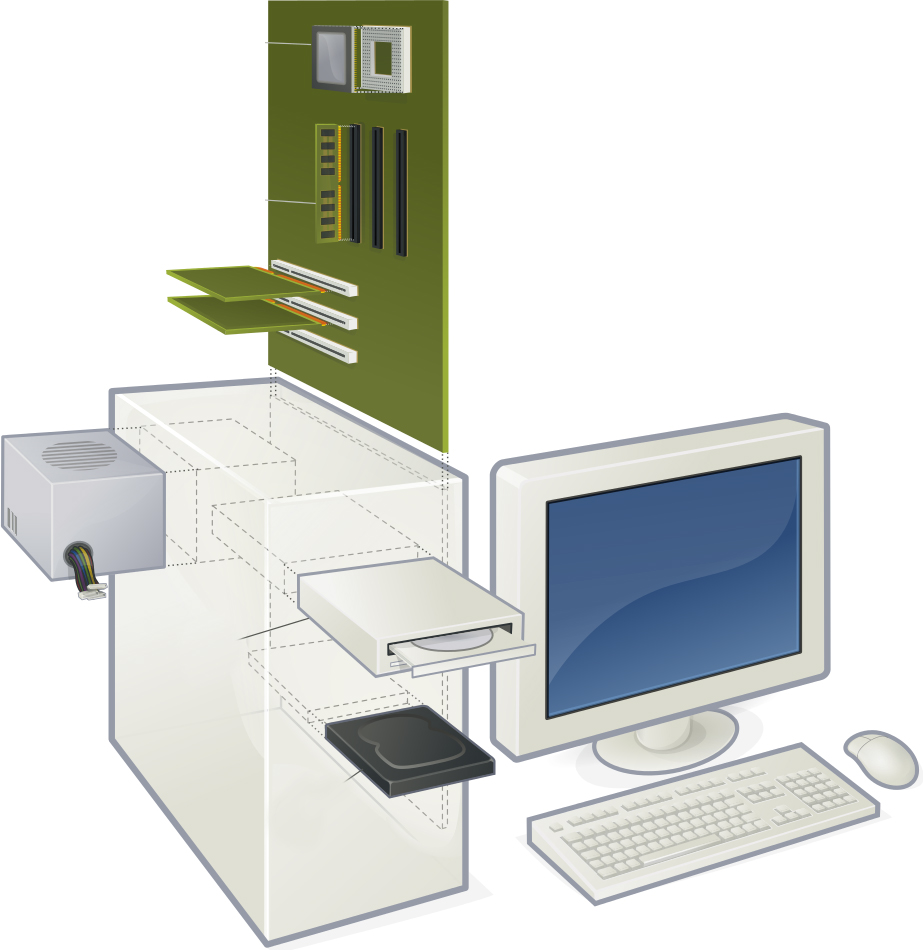
\includegraphics[width=0.3\textwidth]{./Pictures/hardware.jpg}
  \end{center}
  \rule{0.3\textwidth}{0.5pt}
  \caption{Hardware of a modern personal computer}
  \label{fig:hardware}
\end{wrapfigure}
Computer hardware is the collection of physical parts of a computer system. This includes the computer case, monitor, keyboard, and mouse. It also includes all the parts inside the computer case, such as the hard disk drive, motherboard, video card, and many others. Computer hardware is what you can physically touch.

\subparagraph*{Definitions}
\hfill \break
A computer system consists of two major elements: hardware and software. Computer hardware is the collection of all the parts you can physically touch. Computer software, on the other hand, is not something you can touch. Software is a set of instructions for a computer to perform specific operations. You need both hardware and software for a computer system to work.

Some hardware components are easy to recognize, such as the computer case, keyboard, and monitor. However, there are many different types of hardware components. In this lesson, you will learn how to recognize the different components and what they do.


%-----------------------------------
%	SUBSECTION 1
%-----------------------------------
\subsection{Raspberry Pi}
\begin{wrapfigure}{r}{0.5\textwidth}
  \begin{center}
    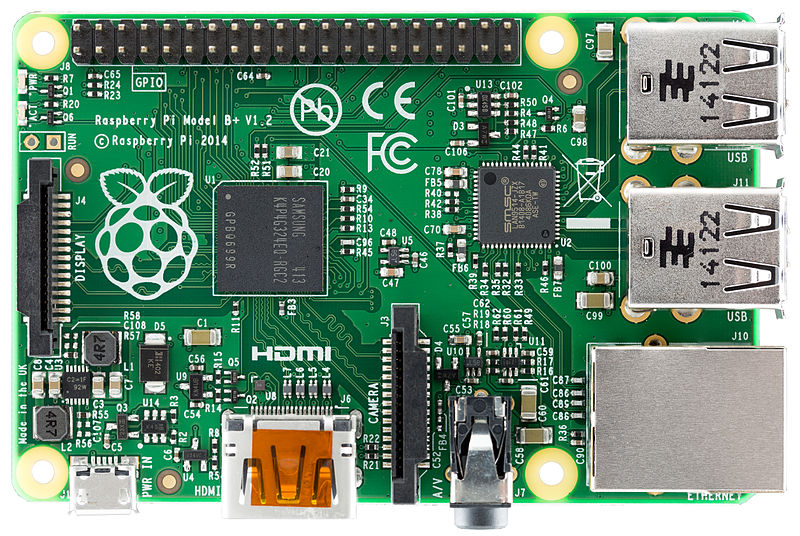
\includegraphics[width=0.5\textwidth]{./Pictures/raspberry_pi_b.jpg}
  \end{center}
  \rule{0.5\textwidth}{0.5pt}
  \caption{Raspberry Pi 1 model B+}
  \label{fig:Raspberry}
\end{wrapfigure}
\paragraph*{A brief history lesson on the Pi}
\hfill \break
Raspberry Pi\footnote{\href{https://www.raspberrypi.org/help/what-is-a-raspberry-pi/}{\texttt{https://www.raspberrypi.org/help/what-is-a-raspberry-pi/}}} (Figure \ref{fig:Raspberry}) is a series of credit card-sized single-board computers developed in the UK by the Raspberry Pi Foundation with the intention of promoting the teaching of basic computer science in schools.

Over the past decades, computers have gotten cheaper and cheaper, so today
you can find them not only at your desk, but also in nearly every consumer
electronics device, such as smartphones and DVD players. Still, computers
aren’t so cheap that you spontaneously buy one when shopping for your
groceries. Usually, you carefully plan your next computer purchase, because
you have to use it for a couple of years.

Computers like the Raspberry Pi will change the situation completely in the
near future. The Raspberry Pi or Pi, for short is a full-blown desktop PC
that costs only \$35. You can connect it directly to the Internet, and it can
display high-definition videos. Also, it runs Linux, so you don’t have to pay
for an operating system. This makes the Pi probably the first throwaway
computer in history.

Originally, the Raspberry Foundation \citep{2} built the Pi to teach children how to
program, so it comes as no surprise that the Pi is an excellent device for
exactly this purpose. 
On top of that, you can use the Pi for many other
exciting things. For example, you can turn it into a multimedia center, use it as a cheap but powerful web server, or play some classic games.
The Pi is also a great machine for experimenting with electronics. In contrast
to many popular microcontroller boards, such as the Arduino, the Pi runs a
full-blown operating system, and you can choose from a wide range of programming
languages to implement your projects.
With cheap and small devices like the Raspberry Pi, a new era of ubiquitous
computing has begun, and you can be part of it.


\paragraph*{ARM}
\hfill \break
A company named Acorn Computers developed a 32-bit RISC architecture named
the Acorn RISC Machine (later renamed to Advanced RISC Machine) in the late
1980s. This architecture proved to be useful beyond their limited product line,
so a company named ARM Holdings was formed to license the architecture for
use in a wide variety of products. It is commonly found in embedded devices
such as cell phones, automobile electronics, MP3 players, televisions, and so on.
The fi rst version of the architecture was introduced in 1985, and at the time of
this writing it is at version 7 (ARMv7). ARM has developed a number of specifi c
cores (e.g., ARM7, ARM7TDMI, ARM926EJS, Cortex)—not to be confused with
the different architecture specifi cations, which are numbered ARMv1–ARMv7.
While there are several versions, most devices are either on ARMv4, 5, 6, or 7.
ARMv4 and v5 are relatively “old,” but they are also the most dominant and
common versions of the processor (“more than 10 billion” cores in existence,
according to ARM marketing). Popular consumer electronic products typically
use more recent versions of the architecture. For example, the third-generation
Apple iPod Touch and iPhone run on an ARMv6 chip, and later iPhone/iPad
and Windows Phone 7 devices are all on ARMv7.\\
\-\hspace{1cm}Whereas companies such as Intel and AMD design and manufacture their
processors, ARM follows a slightly different model. ARM designs the architecture
and licenses it to other companies, which then manufacture and integrate the
processors into their devices. Companies such as Apple, NVIDIA, Qualcomm,
and Texas Instruments market their own processors (A, Tegra, Snapdragon, and OMAP, respectively), but their core architecture is licensed from ARM.\\
\-\hspace{1cm}They all implement the base instruction set and memory model defi ned in the
ARM architecture reference manual. Additional extensions can be added to
the processor; for example, the Jazelle extension enables Java bytecode to be
executed natively on the processor. The Thumb extension adds instructions
that can be 16 or 32 bits wide, thus allowing higher code density (native ARM
instructions are always 32 bits in width). The Debug extension allows engineers
to analyze the physical processor using special debugging hardware. Each
extension is typically represented by a letter (J, T, D, etc.). Depending on their
requirements, manufacturers can decide whether they need to license these
additional extensions. This is why ARMv6 and earlier processors have letters
after them (e.g., ARM1156T2 means ARMv6 with Thumb-2 extension). These
conventions are no longer used in ARMv7, which instead uses three profi les
(Application, Real-time, and Microcontroller) and model name (Cortex) with
different features. For example, ARMv7 Cortex-A series are processors with
the application profi le; and Cortex-M are meant for microcontrollers and only
support Thumb mode execution.

\paragraph*{Get to Know the Hardware}

\begin{wrapfigure}{r}{0.5\textwidth}
\vspace{15pt}
  \begin{center}
    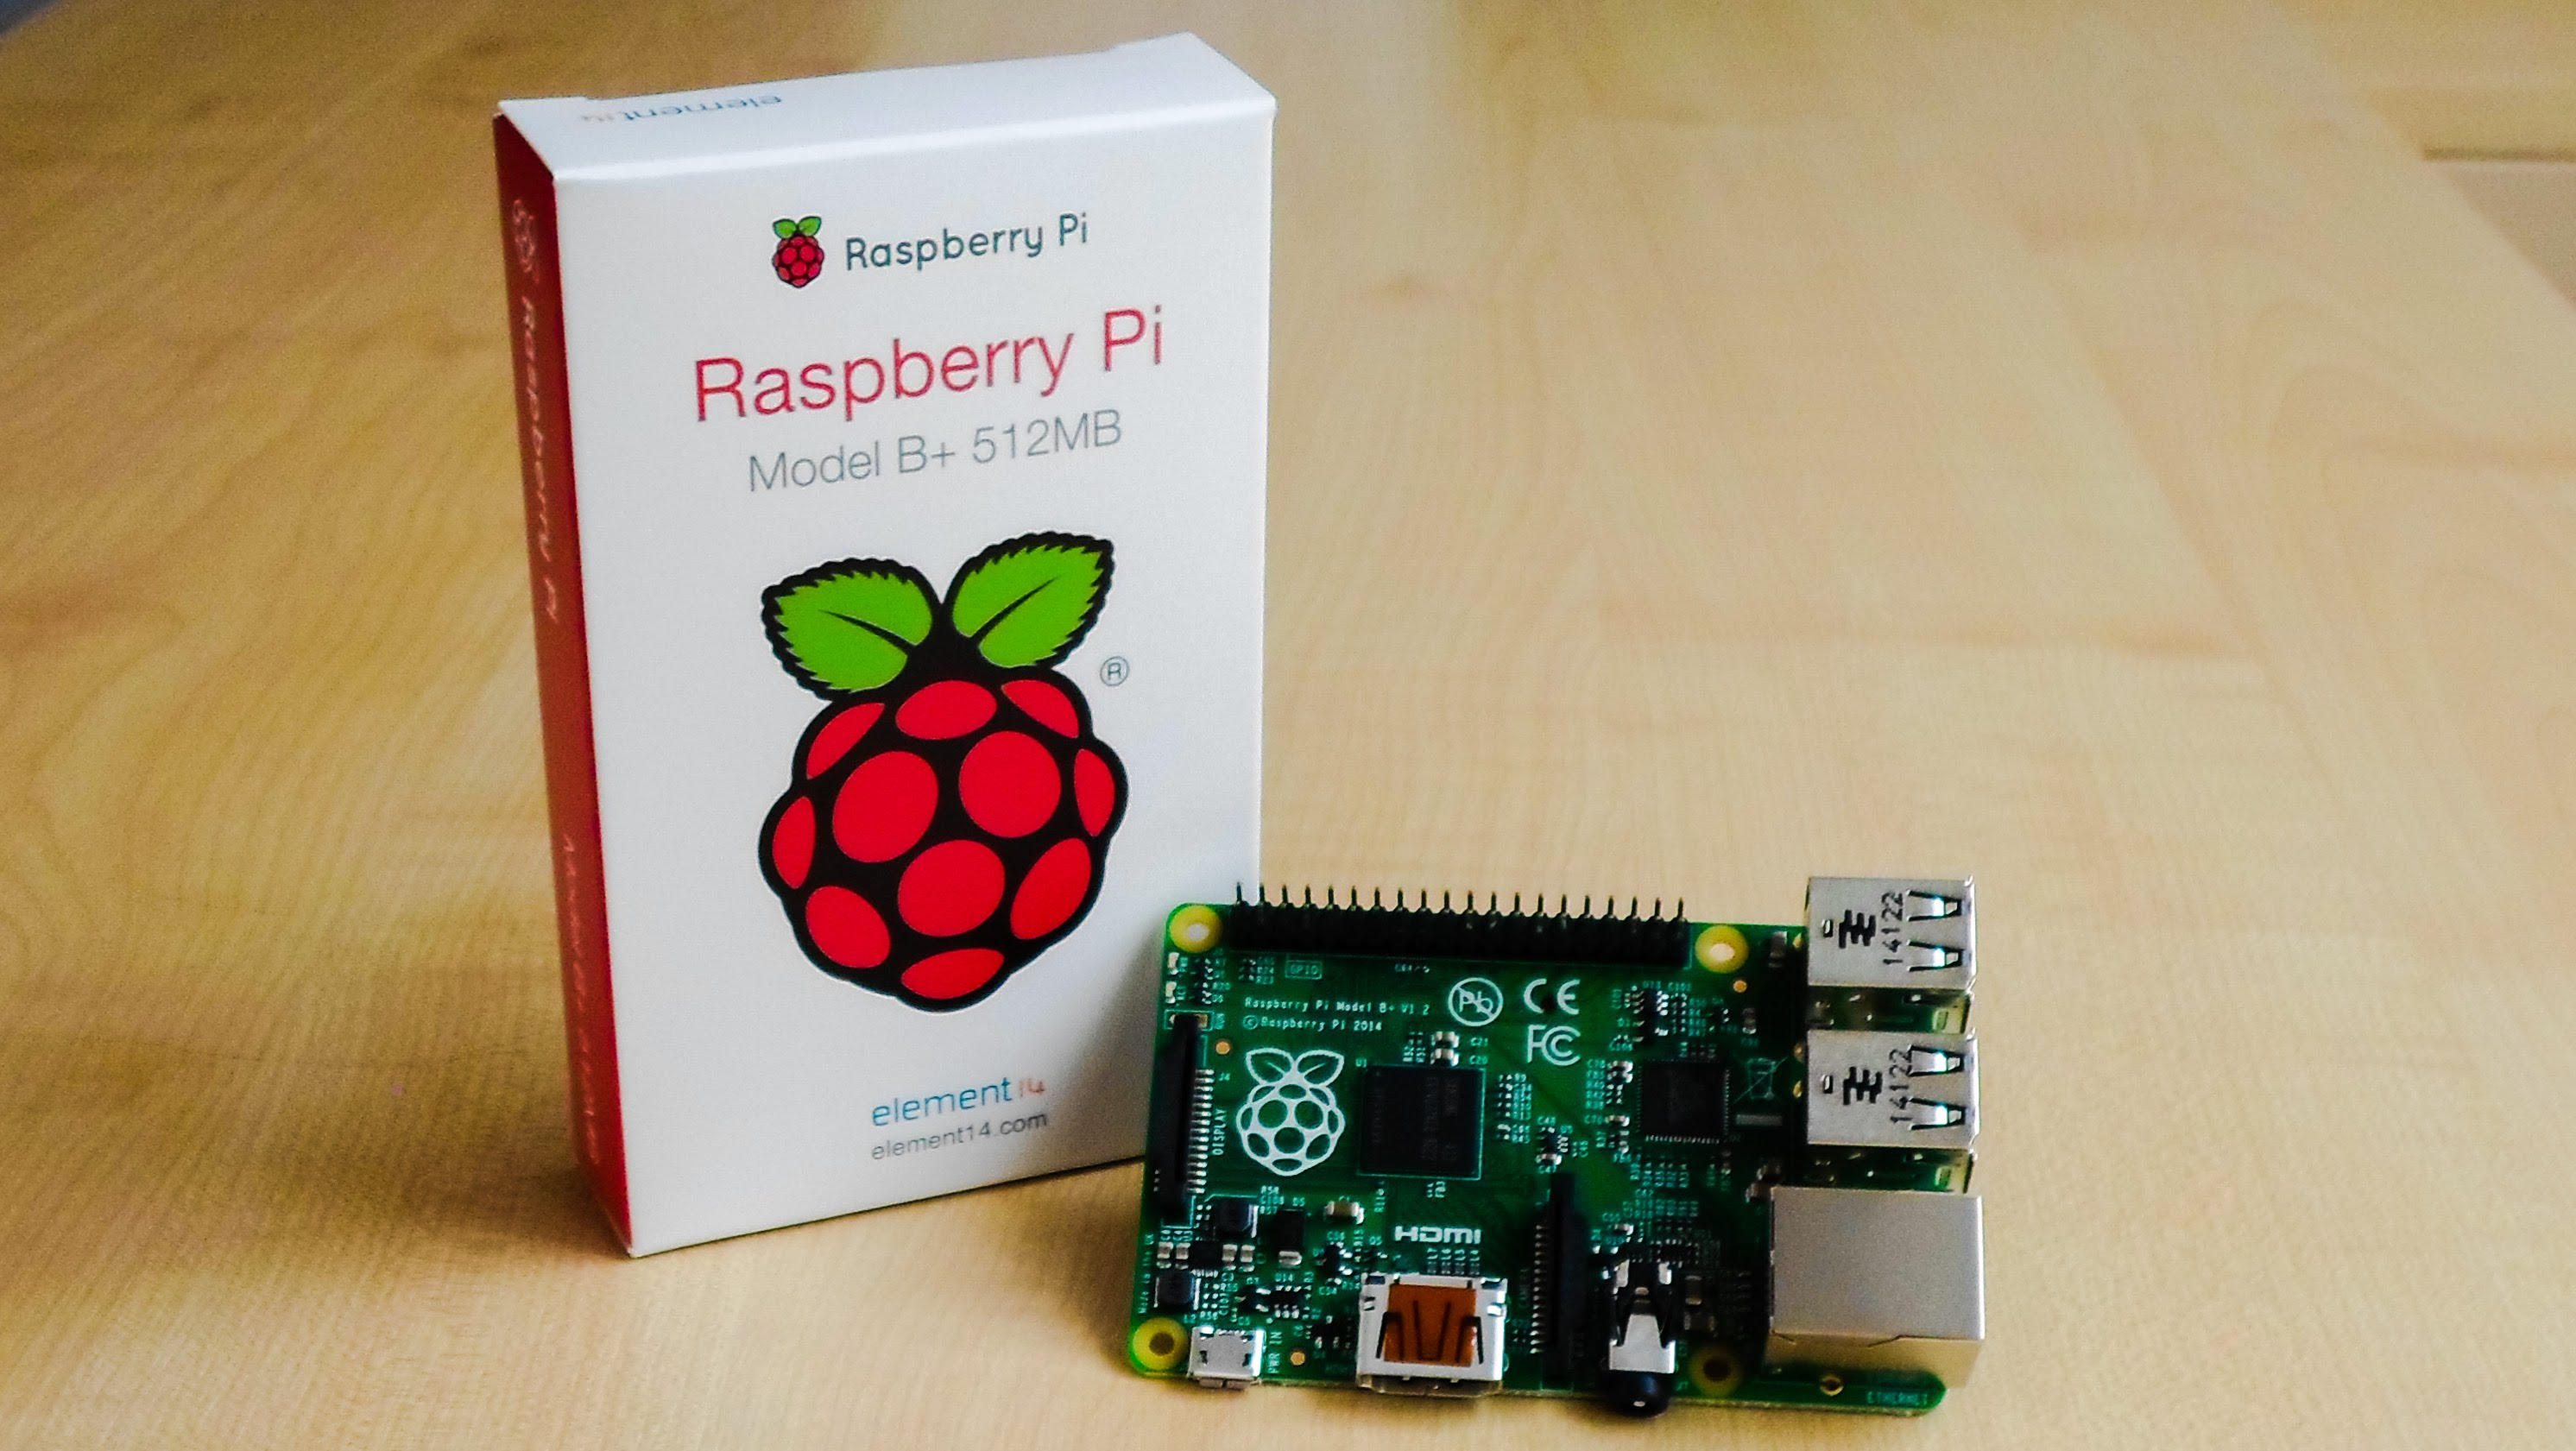
\includegraphics[width=0.5\textwidth]{./Pictures/unboxing_pi.jpg}
  \end{center}
  \rule{0.5\textwidth}{0.5pt}
  \caption{Raspberry Pi }
  \label{fig:unboxing_pi}
\end{wrapfigure}

\hfill \break
Unboxing a new Pi is exciting, but it certainly is not comparable to unboxing
a new Apple product. Usually, the Pi comes in a plain cardboard box with
one or two sheets of paper containing the usual safety hints for electronic
devices and a quick-start guide.

The first version of the Pi looks attractive only to real geeks (Figure \ref{fig:unboxing_pi}). It is a singleboard
computer without a case, and it’s the size of a credit card. It somewhat
resembles the innards of the many electronic devices you might have opened
when you were a child.

\paragraph*{What’s on the Pi}
\hfill \break
At the heart of the Pi is the Broadcom BCM2835 System-on-a-Chip—imagine all the
common hardware components of a PC baked into a small chip. The CPU is called
ARM1176JZF-S, runs at 700 MHz and belongs to the ARM11 family of the ARMv6
architecture. For graphics, the Pi sports a Broadcom VideoCore IV GPU, which is
quite powerful for such a tiny device and capable of full HD video playback. The
following figure (taken from http://www.raspberrypi.org/faqs) shows the
Raspberry Pi model:
\begin{figure}[h!]
  \centering
    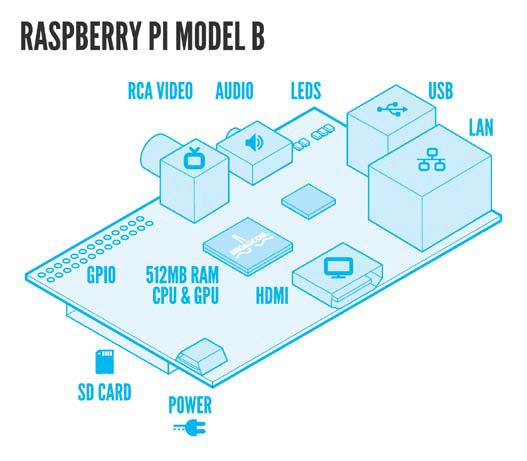
\includegraphics[width=0.5\textwidth]{./Pictures/raspberry_pi_b2.jpg}
  \rule{0.7\textwidth}{1pt}
 \caption{Raspberry Pi Model B board showing key components}
\end{figure}

\subparagraph*{GPIO}
\hfill \break
At the edge of the board we find the General Purpose Input/Output (GPIO) pins,
which, as the name implies, can be used for any kind of general tinkering and to
interface with other pieces of hardware.

\subparagraph*{RCA video}
\hfill \break
This jack is for composite video output, which we can use to connect the Pi to one of
those old television sets using an RCA connector cable.

\subparagraph*{Audio}
\hfill \break
To get sound out of the Pi, we can either get it through the HDMI cable connected
to a monitor, or from this 3.5 mm analog audio jack using headphones or
desktop speakers.

\subparagraph*{LEDs}
\hfill \break
Five status LEDs are used to tell us what the Pi is up to at the moment. They are
as follows:
\begin{itemize}
  \item The green light on top labeled OK (on the older Pi) or ACT (on the newer Pi)
will blink when the Pi is accessing data from the SD card
  \item The light below, labeled PWR, should stay solid red as long as the Pi
has power
  \item The three remaining LEDs will light up when a network cable is connected
to the Ethernet port
\end{itemize}

\subparagraph*{USB}
\hfill \break
The two USB 2.0 ports allow us to connect keyboards, mice, and most importantly
for us, Wi-Fi dongles, microphones, video cameras, and GPS receivers. We can also
expand the number of USB ports available with the help of a self-powered USB hub.

\subparagraph*{LAN}
\hfill \break
The Ethernet LAN port allows us to connect the Pi to a network at a maximum speed
of 100 Mbit/s. This will most commonly be a home router or a switch, but it can also
be connected directly to a PC or a laptop. A Category 5 twisted-pair cable is used for
wired network connections.

\subparagraph*{HDMI}
\hfill \break
The High-Definition Multimedia Interface (HDMI) connector is used to connect the
Pi to a modern TV or monitor. The cable can carry high-resolution video up to 1920 x
1200 pixels and digital sound. It also supports a feature called Consumer Electronics
Control (CEC), which allows us to use the Pi as a remote control for many common
television sets.

\subparagraph*{Power}
\hfill \break
The power input on the Raspberry Pi is a 5V (DC) Micro-USB Type B jack. A power
supply with a standard USB to micro-USB cable, such as a common cellphone
charger, is then connected to feed the Pi.

\subparagraph*{Raspbian OS}

\begin{wrapfigure}{r}{0.4\textwidth}
\vspace{-25pt}
  \begin{center}
    
\includegraphics[width=0.4\textwidth]{./Pictures/raspbian.png}
  \end{center}
\end{wrapfigure}
\hfill \break
Computers can't do anything useful without an operating system, and the Pi is
no exception. There is a growing collection of operating systems available for
the Pi, but we'll stick with the "officially recommended" OS—the Raspbian
GNU/Linux distribution.
\clearpage
%-----------------------------------
%	SUBSECTION 2
%-----------------------------------

\subsection{Car Chassis Development Kit}

Morbi rutrum odio eget arcu adipiscing sodales. Aenean et purus a est pulvinar pellentesque. Cras in elit neque, quis varius elit. Phasellus fringilla, nibh eu tempus venenatis, dolor elit posuere quam, quis adipiscing urna leo nec 

\begin{figure}[h!]
        \centering
        \begin{subfigure}[b]{0.5\textwidth}
                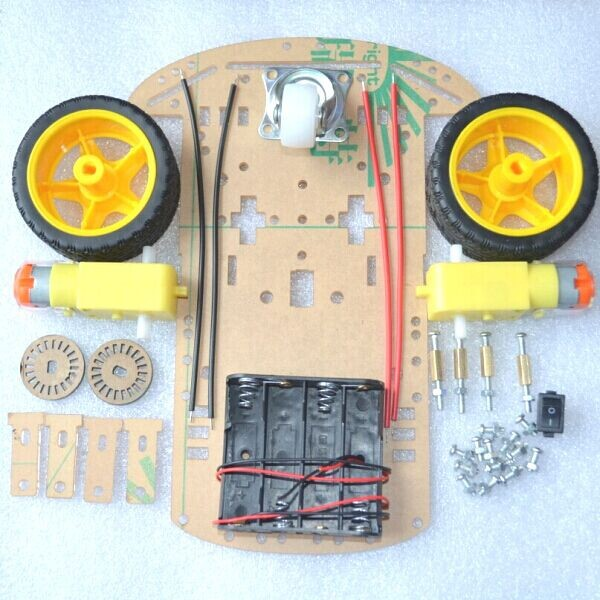
\includegraphics[width=\textwidth]{./Pictures/Car-Chassis-Kit.jpg}
        \end{subfigure}%
        ~ %add desired spacing between images, e. g. ~, \quad, \qquad, \hfill etc.
          %(or a blank line to force the subfigure onto a new line)
        \begin{subfigure}[b]{0.5\textwidth}
                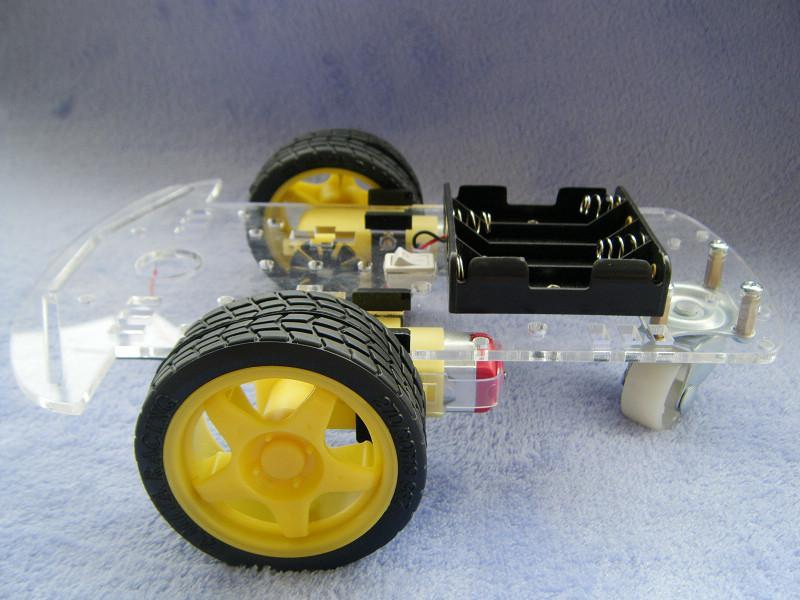
\includegraphics[width=\textwidth]{./Pictures/Car-Chassis-Kit2.jpg}
        \end{subfigure}
        \rule{1\textwidth}{1pt}
        \caption{Car Chassis Development Kit}
\end{figure}
\begin{figure}[h!]
        \centering
        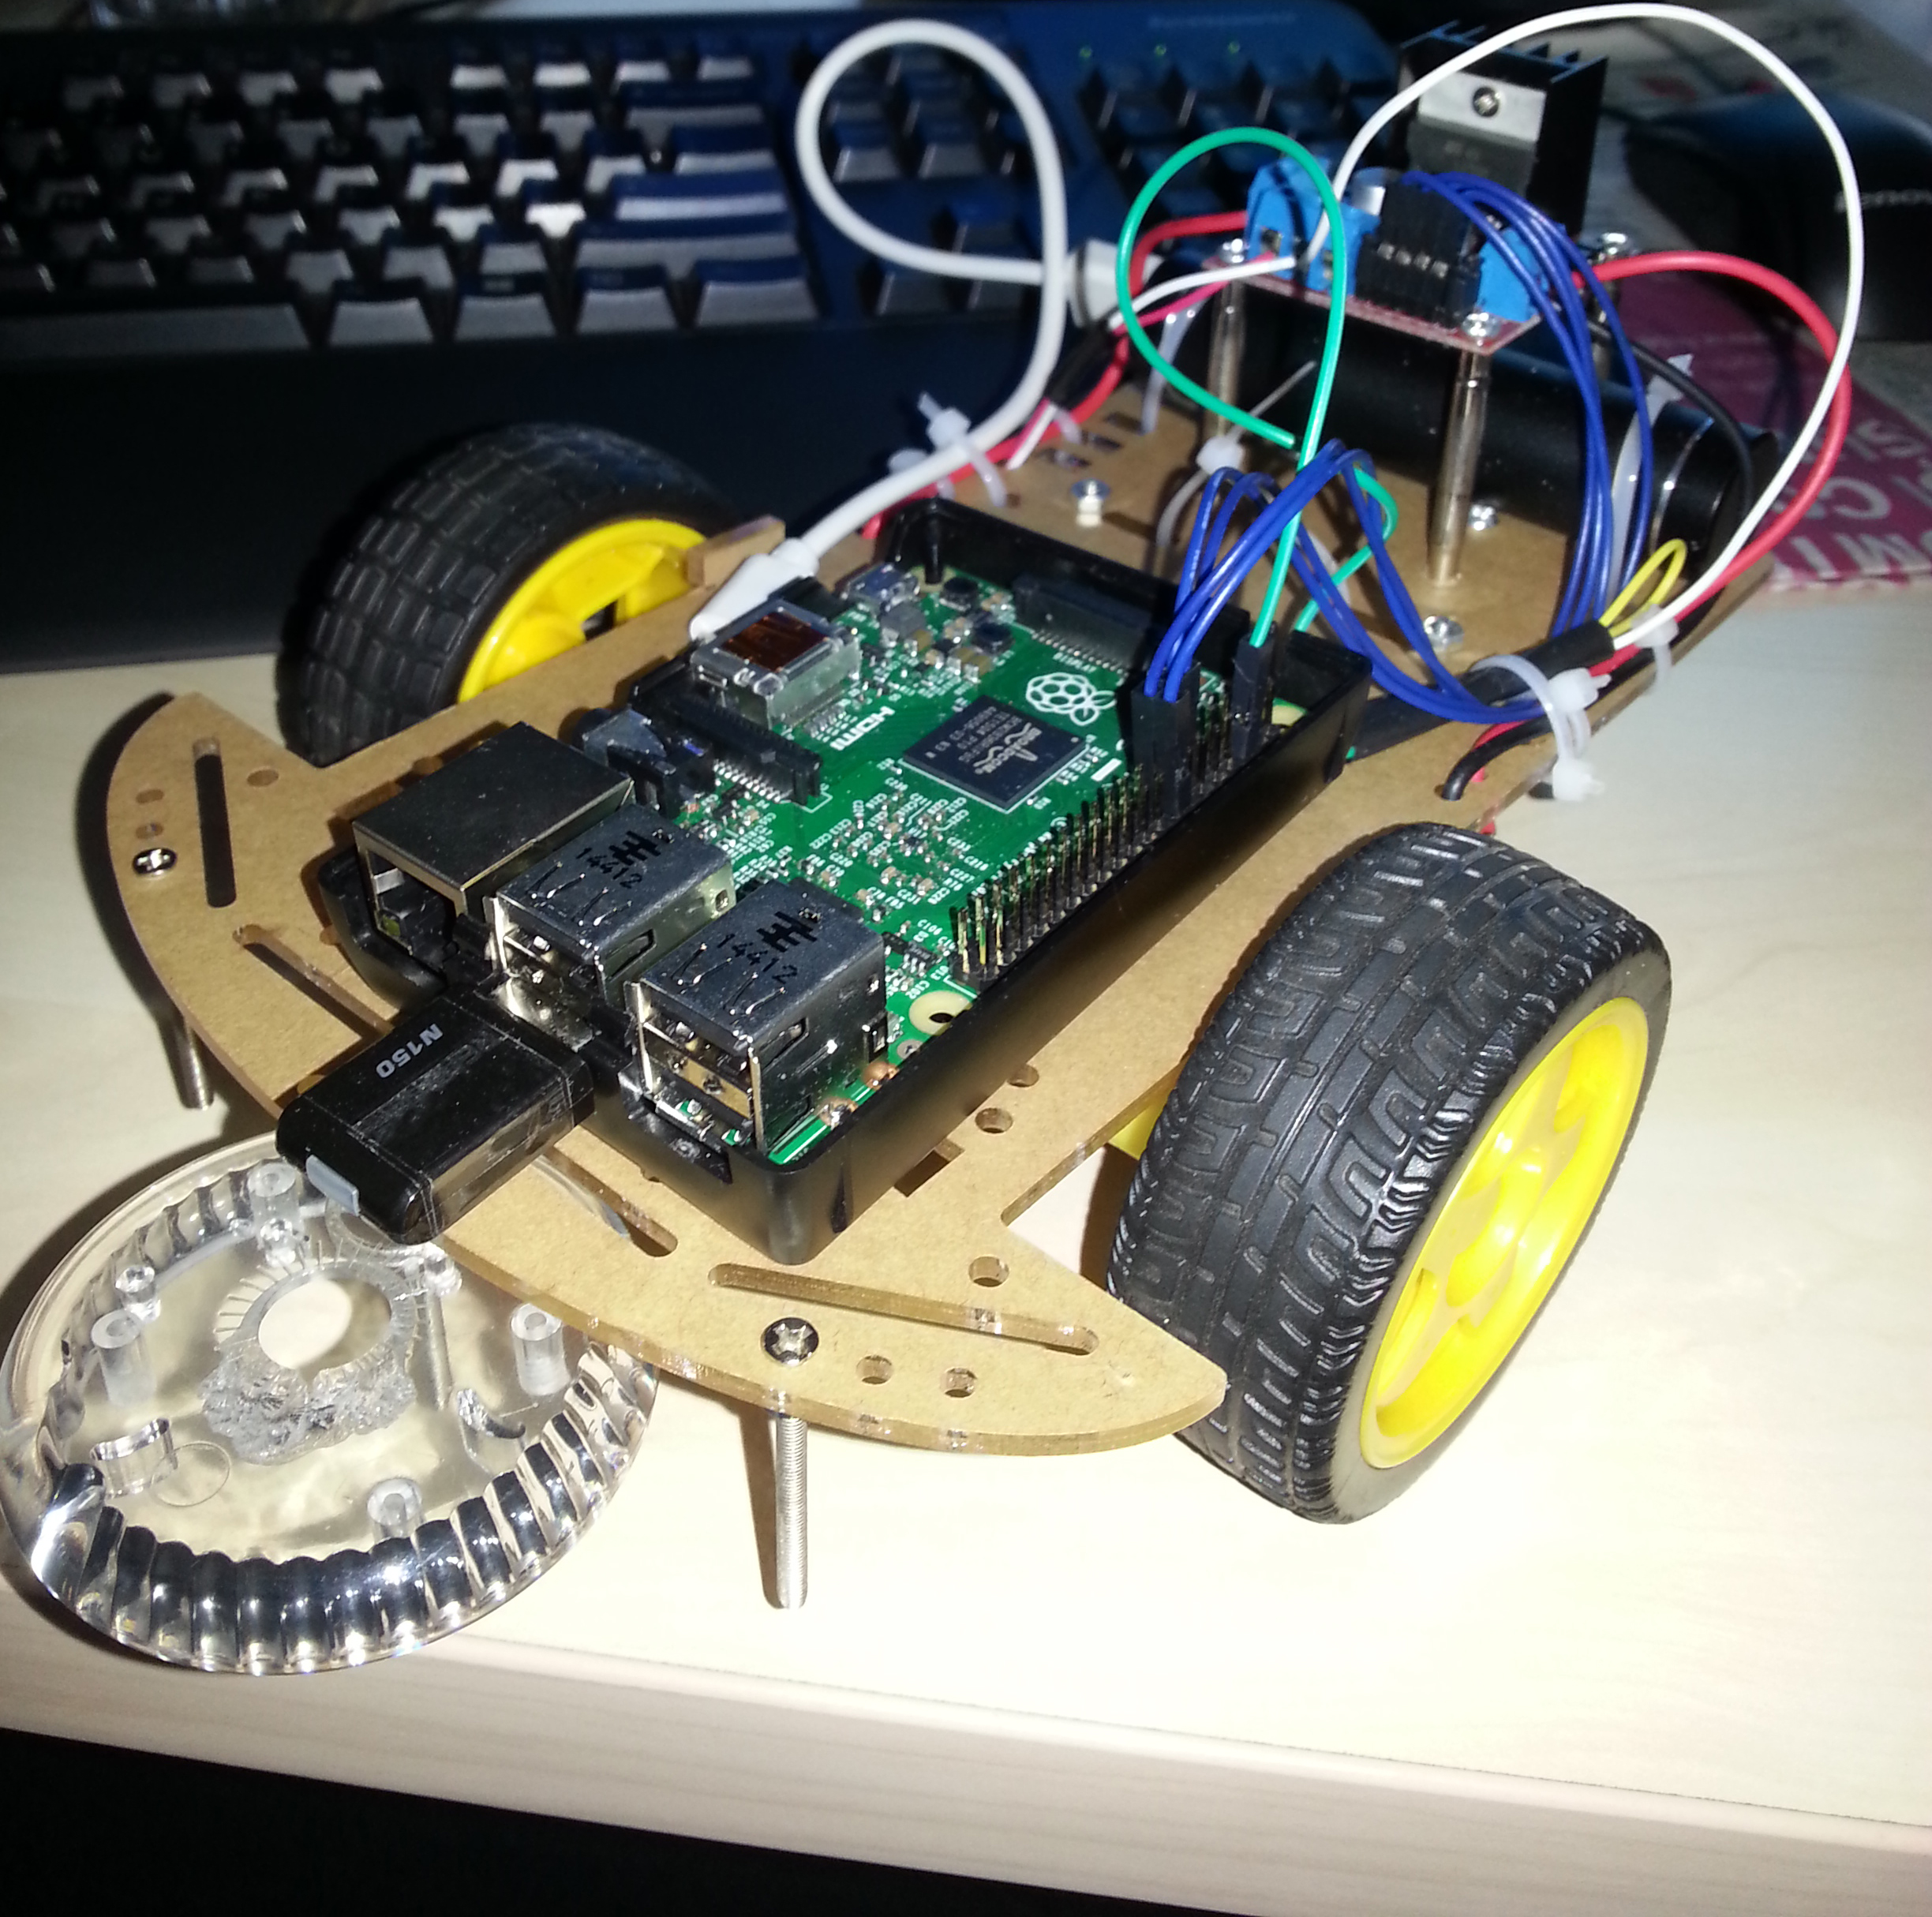
\includegraphics[width=0.5\textwidth]{./Pictures/Car-Chassis-Kit3.jpg}
		\rule{0.5\textwidth}{1pt}
        \caption{Car Chassis Development Kit}
\end{figure}
\clearpage
%----------------------------------------------------------------------------------------
%	SECTION 2
%----------------------------------------------------------------------------------------

\section{Technologies and Programming Languages}

Software is a generic term for organized collections of computer data and instructions, often broken into two major categories: system software that provides the basic non-task-specific functions of the computer, and application software which is used by users to accomplish specific tasks.

System software is responsible for controlling, integrating, and managing the individual hardware components of a computer system so that other software and the users of the system see it as a functional unit without having to be concerned with the low-level details such as transferring data from memory to disk, or rendering text onto a display. Generally, system software consists of an operating system and some fundamental utilities such as disk formatters, file managers, display managers, text editors, user authentication (login) and management tools, and networking and device control software.

Application software, on the other hand, is used to accomplish specific tasks other than just running the computer system. Application software may consist of a single program, such as an image viewer; a small collection of programs (often called a software package) that work closely together to accomplish a task, such as a spreadsheet or text processing system; a larger collection (often called a software suite) of related but independent programs and packages that have a common user interface or shared data format, such as Microsoft Office, which consists of closely integrated word processor, spreadsheet, database, etc.; or a software system, such as a database management system, which is a collection of fundamental programs that may provide some service to a variety of other independent applications.

Software is created with programming languages and related utilities, which may come in several of the above forms: single programs like script interpreters, packages containing a compiler, linker, and other tools; and large suites (often called Integrated Development Environments) that include editors, debuggers, and other tools for multiple languages. 


\paragraph*{Programming Languages}
\hfill \break
There exists an enormous variety of programming languages in use today. Testimony of this fact are the 650 plus different programming languages listed in Wikipedia \footnote{\href{http://en.wikipedia.org/wiki/List_of_programming_languages}{\texttt{List of programming languages}}}. A good understanding of this great diversity is important for many reasons. First, it opens new perspectives to the computer scientist. Problems at first hard in one language might have a very easy solution in another. Thus, knowing which language to use in a given domain might decrease considerably the effort to build an application.



\subparagraph*{What is a Programming Languages}
\hfill \break
A programming language is an artificial language that can be used to instruct a computer to do a particular task. To be considered a general programming language, it must be computationally complete, or Turing-Complete. It is nevertheless common to regard some languages that are not computationally complete, like database query languages and other domain-specific languages as programming languages as well.

\subparagraph*{High-Level Versus Low-Level Programming Languages}
\hfill \break
A low-level programming language is one that is very basic and close to the machine's native language. A low-level programming language can be thought of as a building block language for software. Assembly code is the most common low-level language and requires very little translation to assemble it to machine code. (The 1's and 0's that make up binary.)

A high-level programming language is one that is closer to a level of human communication. In this method, the compiler does a lot more of the work for the programmer. The closer the language is to our everyday speech, the easier it is to worry about more complex problems. However, this can be taken too far. If a language is too much like English (or other natural languages), it can be harder to create complex programs. This is because verbose languages take more time to read, and so they can take a lot more time to understand.
\begin{figure}[h!]
        \centering
                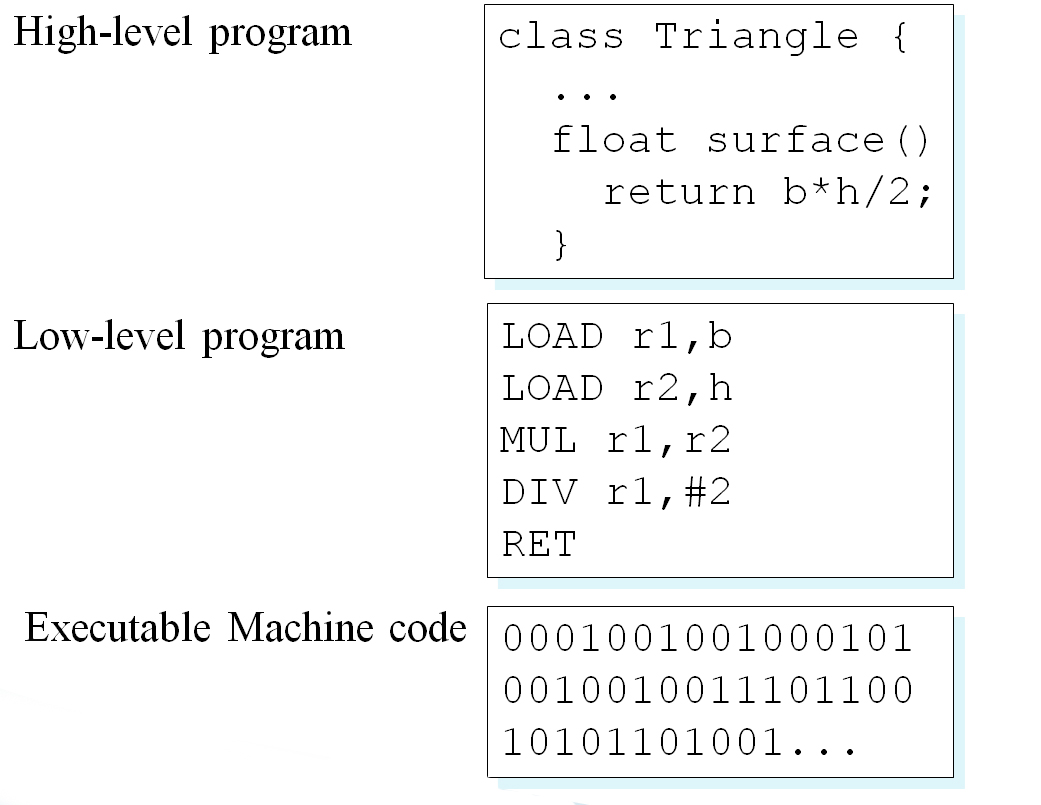
\includegraphics[width=0.7\textwidth]{./Pictures/lavels.jpg}
                  \rule{0.7\textwidth}{1pt}
        \caption{Levels of Programming Languages}
\end{figure}

Machine code is the language the computer can understand directly. Machine code consists of sequences of binary digits. It is almost never programmed in directly, but anything that is to be run on an ordinary computer must be translated to machine code first. The machine code can be different for each computer architecture.

Assembly language is a more human readable representation of the machine code, where the machine instructions are represented as mnemonics rather than binary digits. Assembly language has a 1:1 relationship with machine code as long as the program is not self-modifying. Before an assembly program can be run by a computer, it must be transformed to machine code. A program that does this translation is known as an assembler. In the early days of computing, assembly language was extensively used, but today it is mainly used for very time critical parts of programs, the core of operating systems, as well as in very small computers, like the chip on a smartcard.

Machine code and assembly language are called first and second generation programming languages respectively. A programming language that has arithmetic expressions, looping constructs, functions, and other constructs that save the programmer from dealing with the machine instructions directly is known as a third-generation programming language.

High-level, domain-specific programming languages were earlier often mentioned as fourth-generation languages, while expert systems were called fifth-generation programming languages. In later years this distinction has blurred, as many very high-level general purpose programming languages like Python, Haskell and Common Lisp have emerged. Expert systems are in very little use today.

\subparagraph*{Compilation and interpretation of computer programs}
\hfill \break
Before a program can be executed on a computer, it must be translated to machine code. Alternatively it can be simulated by another program, called an interpreter. A compiler is a program that translates a programming language, called the source programming language into another programming language, called the destination language. Usually the source language is a high level language, while the destination language is machine code. An interpreter may require that the source programming language be compiled into an intermediate form before interpretetion, called byte code. This is a more low level language, for which it is easier to write an interpreter. In the Java programming language this is a separate step, while in other cases it is performed as an integral part of the interpreter. Examples of such programming languages are Perl and Python. CommonLisp is an exception to the above: it's both interpreted and compiled.

\subparagraph*{Type Systems}
\hfill \break
There are two axes to type systems: Dynamic versus Static on the one side and Strong versus Weak.

\begin{itemize}
  \item A Strongly typed language will not allow an operation on an object if this object does not match in type. Examples are CommonLisp, Q-base and Python.
  \item A Weakly typed language will allow such operations. Examples are C and C++.
  \item TDynamic type languages bind type to value. Staticly typed languages bind it to variable.
\end{itemize}

\subsection{Web Application Back-End}
In software engineering, the terms "front end" and "back end" are distinctions which refer to the separation of concerns between a presentation layer and a data access layer respectively.
The front end is an interface between the user and the back end. The front and back ends may be distributed amongst one or more systems.

In software architecture, there may be many layers between the hardware and end user. Each can be spoken of as having a front end and a back end. The front is an abstraction, simplifying the underlying component by providing a user-friendly interface.

In software design, for example, the model-view-controller architecture provides front and back ends for the database, the user and the data processing components. The separation of software systems into front and back ends simplifies development and separates maintenance. A rule of thumb is that the front (or "client") side is any component manipulated by the user. The server-side (or "back end") code resides on the server. The confusion arises when one must make front-end edits to server-side files. Most HTML designers, for instance, don't need to be on the server when they are developing the HTML; conversely, the server-side engineers are, by definition, never on anything but a server. It takes both to ultimately make a functioning, interactive website.
\subsubsection{JavaScript}
JavaScript is the programming language of the Web. The overwhelming majority of
modern websites use JavaScript, and all modern web browsers—on desktops, game
consoles, tablets, and smart phones—include JavaScript interpreters, making JavaScript
the most ubiquitous programming language in history. JavaScript is part of the
triad of technologies that all Web developers must learn: HTML to specify the content
of web pages, CSS to specify the presentation of web pages, and JavaScript to specify
the behavior of web pages. This book will help you master the language.
If you are already familiar with other programming languages, it may help you to know
that JavaScript is a high-level, dynamic, untyped interpreted programming language
that is well-suited to object-oriented and functional programming styles. JavaScript
derives its syntax from Java, its first-class functions from Scheme, and its prototypebased
inheritance from Self. But you do not need to know any of those languages, or
be familiar with those terms, to use this book and learn JavaScript.

The name “JavaScript” is actually somewhat misleading. Except for a superficial syntactic
resemblance, JavaScript is completely different from the Java programming language.
And JavaScript has long since outgrown its scripting-language roots to become
a robust and efficient general-purpose language. The latest version of the language (see
the sidebar) defines new features for serious large-scale software development.

\paragraph*{JavaScript: Names and Versions}
\hfill \break
JavaScript was created at Netscape in the early days of the Web, and technically, “JavaScript”
is a trademark licensed from Sun Microsystems (now Oracle) used to describe
Netscape’s (now Mozilla’s) implementation of the language. Netscape submitted the
language for standardization to ECMA—the European Computer Manufacturer’s Association—and
because of trademark issues, the standardized version of the language
was stuck with the awkward name “ECMAScript.” For the same trademark reasons,
Microsoft’s version of the language is formally known as “JScript.” In practice, just
about everyone calls the language JavaScript. This book uses the name “ECMAScript”
only to refer to the language standard.


For the last decade, all web browsers have implemented version 3 of the ECMAScript
standard and there has really been no need to think about version numbers: the language
standard was stable and browser implementations of the language were, for the
most part, interoperable. Recently, an important new version of the language has been
defined as ECMAScript version 5 and, at the time of this writing, browsers are beginning
to implement it. This book covers all the new features of ECMAScript 5 as well as all
the long-standing features of ECMAScript 3. You’ll sometimes see these language versions
abbreviated as ES3 and ES5, just as you’ll sometimes see the name JavaScript
abbreviated as JS.


When we’re speaking of the language itself, the only version numbers that are relevant
are ECMAScript versions 3 or 5. (Version 4 of ECMAScript was under development
for years, but proved to be too ambitious and was never released.) Sometimes, however,
you’ll also see a JavaScript version number, such as JavaScript 1.5 or JavaScript 1.8.
These are Mozilla’s version numbers: version 1.5 is basically ECMAScript 3, and later
versions include nonstandard language extensions. Finally, there are
also version numbers attached to particular JavaScript interpreters or “engines.” Google
calls its JavaScript interpreter V8, for example, and at the time of this writing the
current version of the V8 engine is 3.0.


\paragraph*{Exploring JavaScript}
\hfill \break
When learning a new programming language, it’s important to try the examples in the
book, and then modify them and try them again to test your understanding of the
language. To do that, you need a JavaScript interpreter. Fortunately, every web browser
includes a JavaScript interpreter, and if you’re reading this book, you probably already
have more than one web browser installed on your computer.

We’ll see later on in this chapter that you can embed JavaScript code within <script>
tags in HTML files, and when the browser loads the file, it will execute the code. Fortunately,
however, you don’t have to do that every time you want to try out simple
snippets of JavaScript code. Spurred on by the powerful and innovative Firebug extension
for Firefox (pictured in Figure \ref{fig:Firebug} and available for download from \href{http://getfirebug.com/}{http://getfirebug.com/}, today’s web browsers all include web developer tools that are indispensable for
debugging, experimenting, and learning. You can usually find these tools in the Tools
menu of the browser under names like “Developer Tools” or “Web Console.”
(Firefox 4 includes a built-in “Web Console,” but at the time of this writing, the Firebug
extension is better.) Often, you can call up a console with a keystroke like F12 or Ctrl-Shift-J.
These console tools often appear as panes at the top or bottom of the browser
window, but some allow you to open them as separate windows (as pictured in Figure
\ref{fig:Firebug}), which is often quite convenient.


A typical “developer tools” pane or window includes multiple tabs that allow you to
inspect things like HTML document structure, CSS styles, network requests, and so
on. One of the tabs is a “JavaScript console” that allows you to type in lines of JavaScript
code and try them out. This is a particularly easy way to play around with JavaScript,
and I recommend that you use it as you read this book.

There is a simple console API that is portably implemented by modern browsers. You
can use the function console.log() to display text on the console. This is often surprisingly
helpful while debugging, and some of the examples in this book (even in the
core language section) use console.log() to perform simple output. A similar but more
intrusive way to display output or debugging messages is by passing a string of text to
the alert() function, which displays it in a modal dialog box.
\begin{figure}[h!]
  \centering
    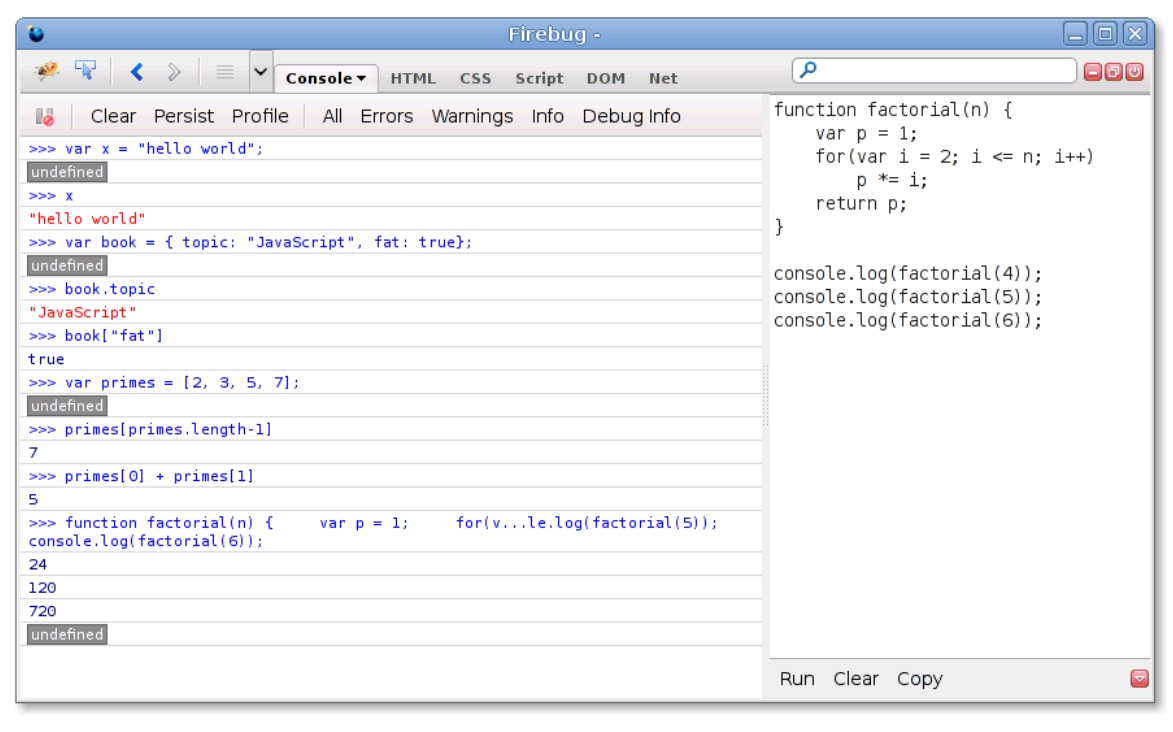
\includegraphics[width=\textwidth]{./Pictures/firebug.jpg}
  \rule{1\textwidth}{1pt}
 \caption{The Firebug debugging console for Firefox}
 \label{fig:Firebug}
\end{figure}


\subsubsection{NodeJs}
Node.js is an open source, cross-platform runtime environment for server-side and networking applications. Node.js applications are written in JavaScript, and can be run within the Node.js runtime on OS X, Microsoft Windows, Linux, FreeBSD, NonStop and IBM i.

Node.js provides an event-driven architecture and a non-blocking I/O API that optimizes an application's throughput and scalability. These technologies are commonly used for real-time web applications.
Node.js uses the Google V8 JavaScript engine to execute code, and a large percentage of the basic modules are written in JavaScript. Node.js contains a built-in library to allow applications to act as a Web server without software such as Apache HTTP Server or IIS.
\paragraph*{History}
\hfill \break
Node.js was invented in 2009 by Ryan Dahl, and other developers working at Joyent. Node.js was created and first published for Linux use in 2009. Its development and maintenance was spearheaded by Ryan Dahl and sponsored by Joyent, the firm where Dahl worked.

Dahl was inspired to create Node.js after seeing a file upload progress bar on Flickr. The browser did not know how much of the file had been uploaded and had to query the Web server. Dahl desired an easier way.

It garnered international attention after its debut at the inaugural European JSConf on November 8, 2009. Dahl presented Node.js, which combined Google's V8 JavaScript engine, an event-loop, and a low-level I/O API. The project received a standing ovation, and has since then experienced significant growth, popularity and adoption.

In 2011, a package manager was introduced for Node.js library, called npm. The package manager allows publishing and sharing of open-source Node.js libraries by the community, and simplifies installation, updating and uninstallation of libraries.

In June 2011, Microsoft partnered with Joyent to implement a native Windows version of Node.js. The first Node.js build to support Windows was released in July.

In January 2012, Dahl stepped aside, promoting coworker and npm creator Isaac Schlueter to manage the project.

In January 2014, Schlueter announced Timothy J. Fontaine would be Node.js's new project lead.

In December 2014, Fedor Indutny started io.js, a fork of Node.js. Due to internal conflict over Joyent's governance, io.js was created as an open governance alternative with a separate technical committee.

\subsubsection{ExpressJs}
Express.js is a Node.js web application framework, designed for building single-page, multi-page, and hybrid web applications.
Express is a minimal and flexible Node.js web application framework that provides a robust set of features for web and mobile applications.
\subsubsection{Socket.io}
Socket.IO enables real-time bidirectional event-based communication.
It works on every platform, browser or device, focusing equally on reliability and speed.
\subsection{Web Application Front-End} 
Front end development is the development of those elements of a website that the customer sees and interacts with directly. It is a combination of programming skills (knowing which program to choose) and aesthetics (understanding element arrangements on the screen, the color and font choices). The challenges associated with front end developers is that the tools and techniques used to create the front end of a website change constantly and so the developer needs to constantly be aware of how the field is developing.
The objective of designing a site is to ensure that when the users open up the site they see the information in a format that is easy to read and relevant. This is further complicated by the fact that users now use a large variety of devices with varying screen sizes and resolutions thus forcing the designer to take into consideration these aspects when designing the site. They need to ensure that their site comes up correctly in different browsers (cross-browser), different operating systems (cross-platform) and different devices (cross-device), which needs careful planning on the site of the developer.
\subsubsection{HTML (HyperText Markup Language)}
\subsubsection{CSS (Cascading Style Sheets)}
\subsubsection{Less}
\subsubsection{CoffeeScript}
\subsubsection{jQuery}
\subsection{Tools Used for Developing}
\subsubsection{Sublime Text 3}
\subsubsection{GruntJs}
\subsubsection{PuTTY}
\subsubsection{Basic UNIX commands}
